%%--------------------------------%
\Chapter{Robot Agility Use Cases}
\label{chapter:DOWNS}
%%--------------------------------% 
As part of the Robotic Systems for Smart Manufacturing Program and specifically the Agility
Performance of Robotic Systems Project, there is a need for use cases that are representative of the
industry’s needs. Thus there is a combined effort to determine these use cases through two different
methods. One is by getting input from industry representatives, while the other is through a literature
review, the results of which are described below.
\section{Non-Assembly Use Cases}
In this Chapter, we present use cases from non-assembly manufacturing operations.
\subsection{Parts Sorting}
Song \textit{et al.}~\cite{Song.2000} used, as an example, a parts sorting task where a set of randomly placed bolts on a conveyor needed to be sorted into separate bins, as shown in Figure~\ref{fig:Tony1}. The robotic workcell in this example consisted of a single robotic manipulator arm, a disc conveyor, and a number of sensors to determine the placement and orientations of the randomly placed bolts. The task requires the manipulator and conveyor’s motion be synchronized and use the sensors to be able to pick and place the bolts.

\begin{figure}[!htb]
\centering
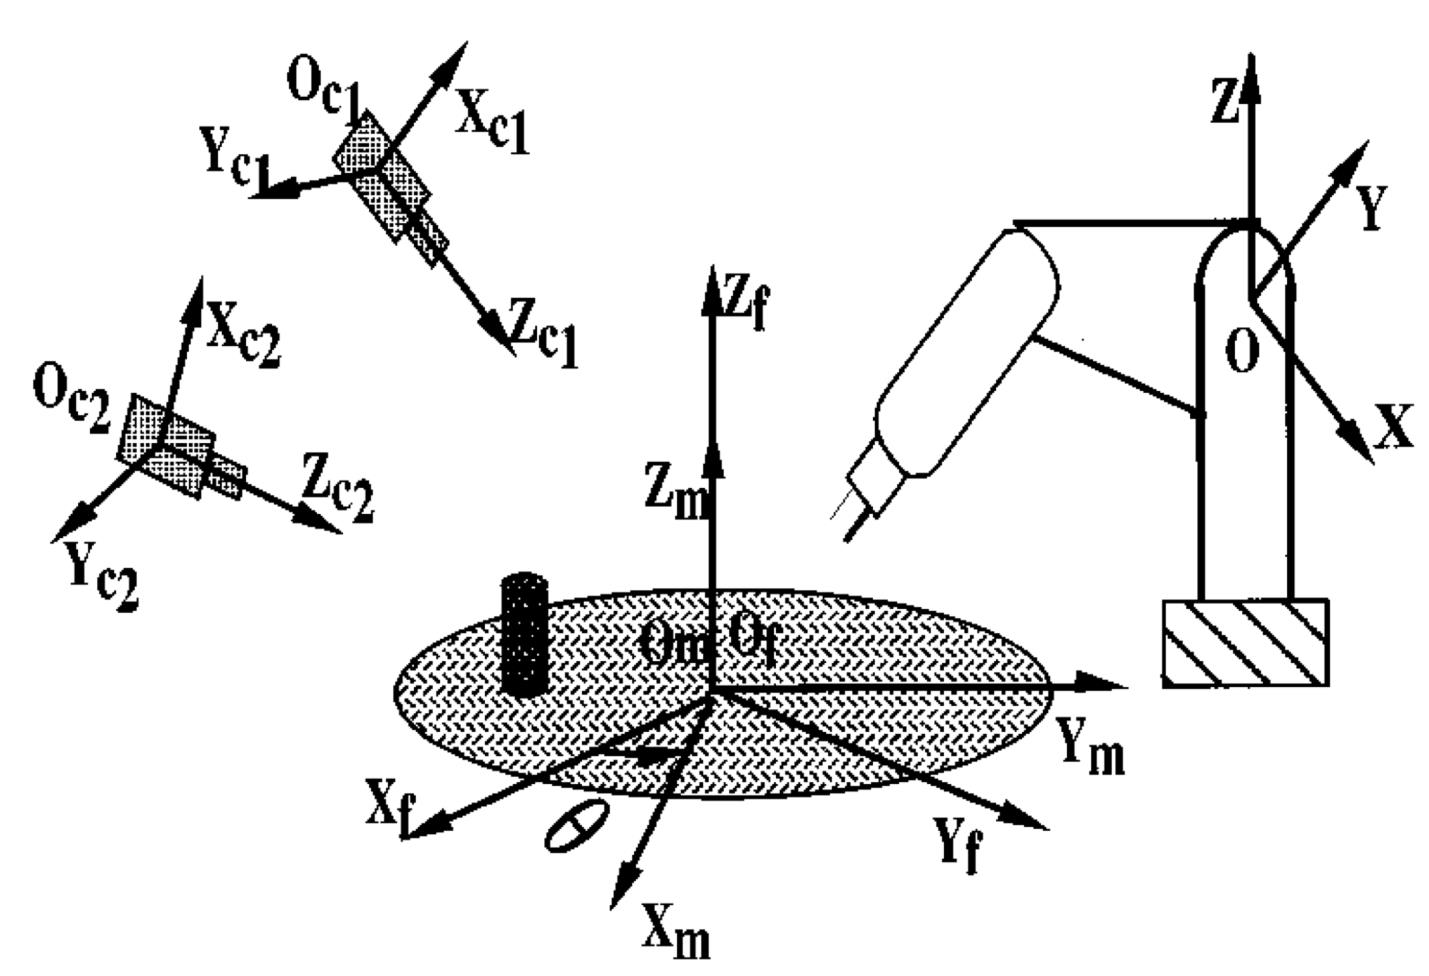
\includegraphics[width=8cm]{Figures/Tony-Fig1.jpg}
\caption{Parts Sorting Task with Robotic Manipulator and Disc Conveyor~\cite{Song.2000}.}
\label{fig:Tony1}
\end{figure}

\subsection{Milling}
\begin{figure}[!htb]
\centering
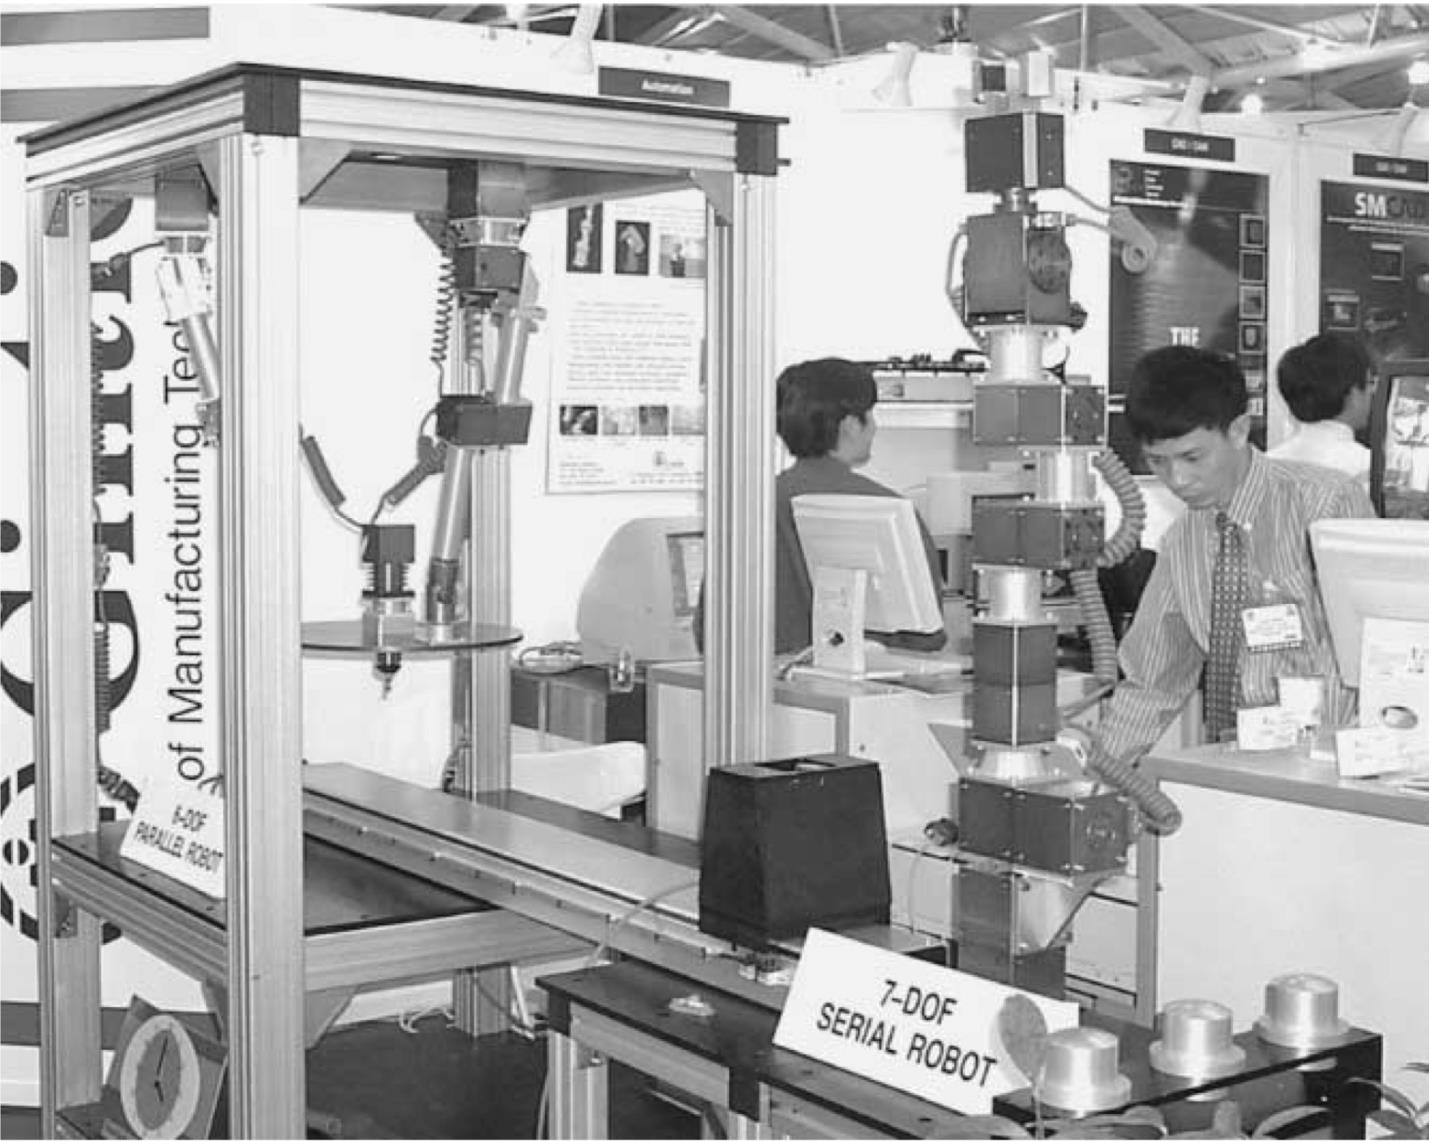
\includegraphics[width=8cm]{Figures/Tony-Fig2.jpg}
\caption{Robotic Milling Operation Use Case~\cite{Chen.2001}.}
\label{fig:Tony2}
\end{figure}

Chen~\cite{Chen.2001} used, as a case study for the reconfigurable workcell, a light machining task involving multiple robots as shown in Figure~\ref{fig:Tony2}. In this case study, the first robot starts by picking up an object and transfers it to the second robot which performs a complete milling operation on a dome-shaped top of a cylindrical workpiece. The first robot then takes the object back and places the milled object into a storage rack. This particular case study could be useful for future focus areas and/or as a use case more focused on collaborative robotics given the multi-robot nature of this example.

\section{Assembly Use Cases}
The following examples fall into the category of assembly-type manufacturing use cases.
\subsection{Snap and Insert}
Quinn \textit{et al.}~\cite{QUINN.1997} used, as an example assembly task for testing their system, a small assembly with four plastic components as shown in Figure~\ref{fig:Tony3}. Part A acts as a base to which parts B, C, and D are attached. Part B gets snapped on to the base, after which the subassembly is inverted. Parts C and D are then inserted into the bottom, with the help of a special guide.  The paper describes this task as a typical light assembly task, perfect for their workcell. The paper describes three cases for division of labor for two robots. Case 1 consists of the two robots performing the complete assembly task in parallel, while Case 2 involves each robot performing part of the assembly task (Robot 1 attaches Part B to Part A, then hands off the sub assembly to Robot 2 to perform the insertion of Parts C and D). Case 3 would consist of Robot 1 feeding the parts to Robot 2, which would perform the assembly.
\begin{figure}[!htb]
\centering
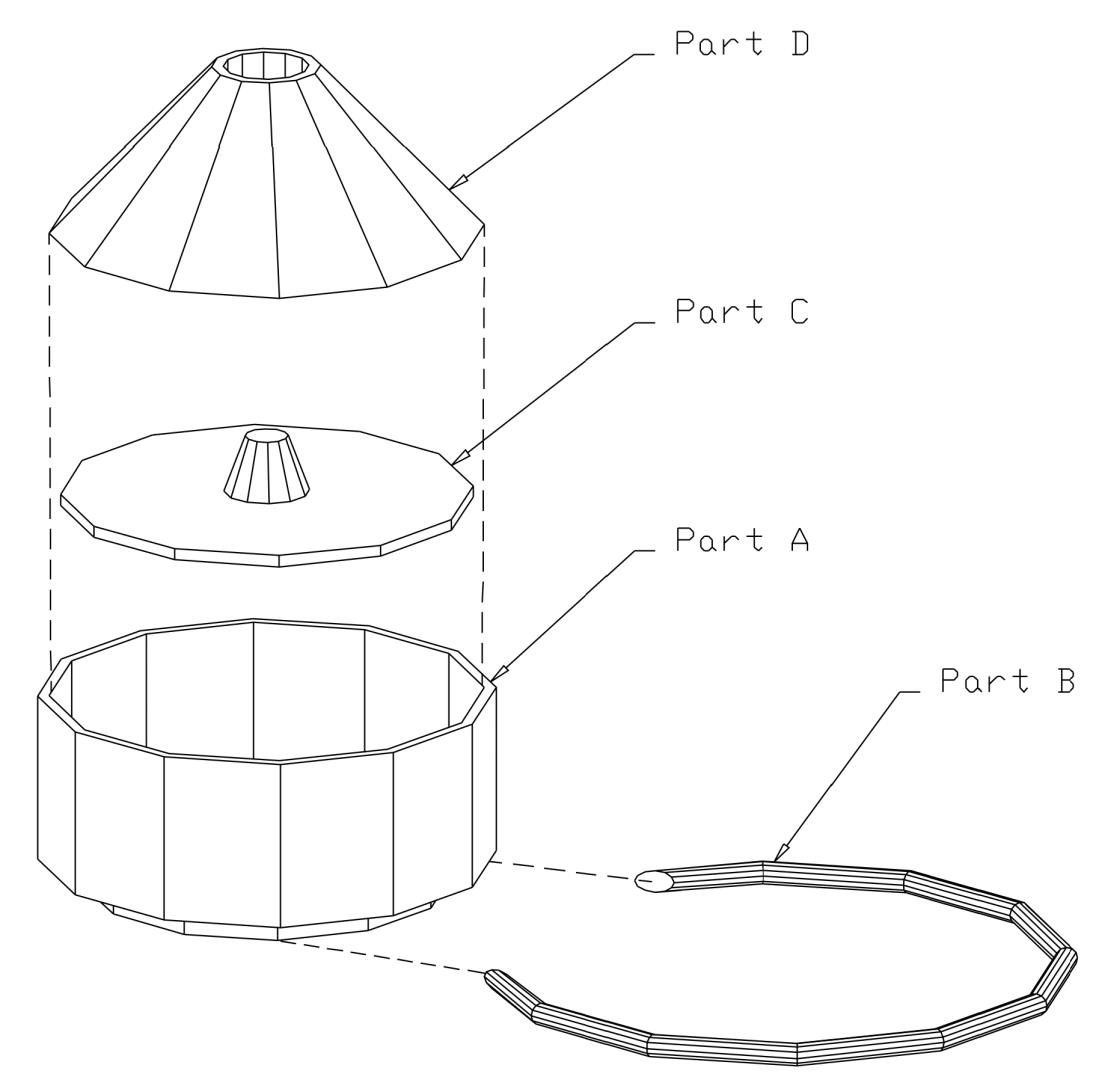
\includegraphics[width=8cm]{Figures/Tony-Fig3.jpg}
\caption{Small Snap and Insert Assembly Containing Four Plastic Parts~\cite{QUINN.1997}.}
\label{fig:Tony3}
\end{figure}
\subsection{Adhesive Tape Roll Dispenser}
Frei and Di Marzo Serugendo~\cite{FREI.2008} used, as an example, an assembly system consisting of body parts (Parts 1 and 3), a tape roll (Part 2) and a screw (Part 4) for locking the body parts together, as shown in Figure~\ref{fig:Tony4}. The case study used consisted of three robots to perform the assembly process. Robot 1 would assemble the Body Parts 1 and 3, while Robot 2 assembles Part 2 and Robot 3 assembles Part 4.
\begin{figure}[!htb]
\centering
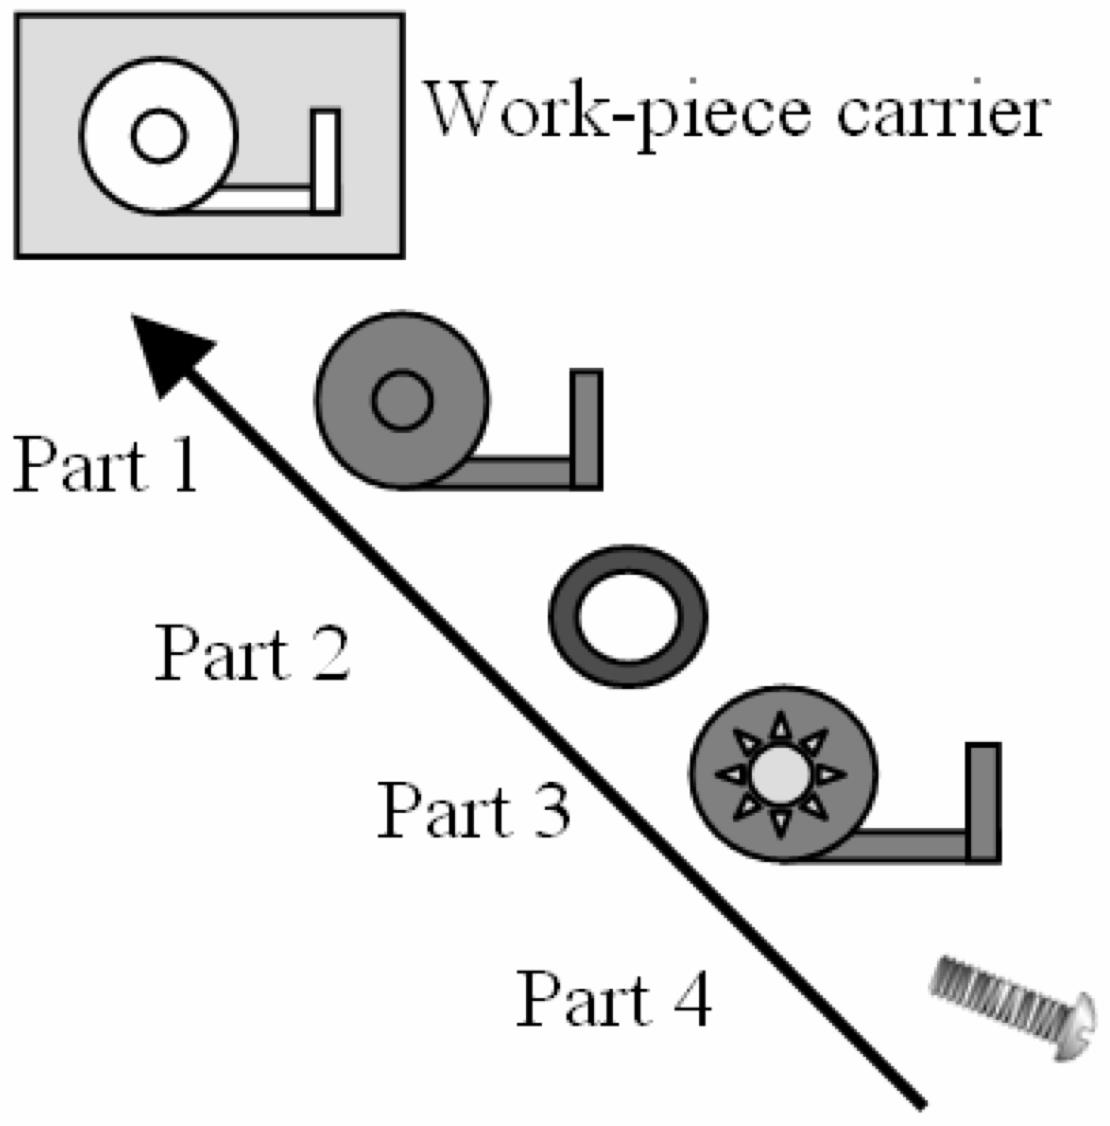
\includegraphics[width=8cm]{Figures/Tony-Fig4.jpg}
\caption{Adhesive Tape Roller Assembly and Kitting Process~\cite{FREI.2008}.}
\label{fig:Tony4}
\end{figure}
\section{Change Cases}
Use cases for changes were also a focus of the literature review. A couple of examples are described below.
\subsection{Adhesive Tape Roll Dispenser}
 Frei and Di Marzo Serugendo~\cite{FREI.2008} proposed a number of scenarios to trigger their self-organization process, as shown in Figure~\ref{fig:Tony5}. The first scenario was to establish a new layout or product order consisting of new user preferences. This would also be the initialization scenario to begin the assembly process. The second scenario would be a change in the locking method from a screw-type to a snap-fit method. This would result in the removal of Part 4 and Robot 4, as well as the need for Robot 1 to be able to apply force to the snap-fit. The third scenario would be a change from a tube of tape rolls to a stick of tape rolls. This would result in Robot 2 needing to switch its method of grabbing the tape roll from expansion to compression.
 \begin{figure}[!htb]
\centering
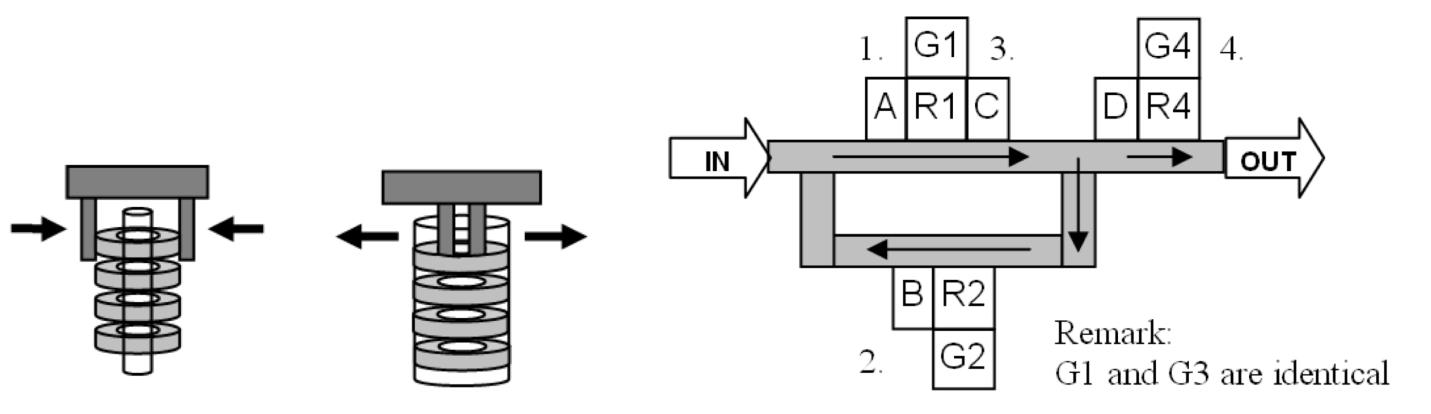
\includegraphics[width=10cm]{Figures/Tony-Fig5.jpg}
\caption{Tape Roll Change Case and Assembly Layout~\cite{FREI.2008}.}
\label{fig:Tony5}
\end{figure}
\subsection{Change Cases for Planning \& Scheduling}
Ling \textit{et al.}~\cite{Ling.1994} used a set of three test cases (one normal situation and two situations where agility was needed to handle disruptions) as part of testing their Planning and Scheduling methodology.  Case 1 was the normal situation and was used as the baseline to measure the changes caused by the other cases. Case 2 involved the introduction of a new high priority order into the system causing a re-prioritization of the existing robotic assembly testbed components. Case 3 involved a machine breakdown, which has a similar effect as Case 2 where a re-prioritization of the existing components must occur to absorb the impact of the broken machinery.  Another re-prioritization would occur when the machine has been repaired and is ready to return to use in the assembly process.
